\documentclass[twocolumn]{svjour3}

\RequirePackage{fix-cm}

\usepackage{wrapfig}

\usepackage{graphicx}
\usepackage{caption}
\usepackage{subcaption}
\captionsetup{compatibility=false}

\usepackage{xcolor}
\usepackage{enumitem,amsmath,amssymb}
\usepackage{breakurl}    % used for \url and \burl
\usepackage[linesnumbered,noline,noend,vlined,ruled]{algorithm2e}
\def\defaultHypSeparation{\hskip.1in}

\usepackage{tikz}
%\usepackage{subfig}
\usepackage{array,booktabs,multirow}
\usepackage{placeins}

\usepackage{logictools}
\usepackage{prooftheory}
\usepackage{comment}
\usepackage{mathenvironments}
\usepackage{drawproof}

\DeclareMathOperator{\pebble}{P}
\DeclareMathOperator{\unpebble}{U}
%\DeclareMathOperator{\pebbledAt}{pebbledAt}
\DeclareMathOperator{\peb}{peb}
\DeclareMathOperator{\free}{free}
\DeclareMathOperator{\ap}{\alpha}
\DeclareMathOperator{\relPerfomance}{rp}
\newcommand{\pebbledAt}[2]{Peb^{#1}_{#2}}
\newcommand{\unpebbleAt}[2]{UPeb^{#1}_{#2}}

\newcommand{\indexIn}[3]{\ensuremath{#1 \scriptstyle \in \{#2\ldots #3\} \displaystyle}}

\usetikzlibrary{patterns}

\renewcommand{\topfraction}{0.85}
\renewcommand{\textfraction}{0.1}
\renewcommand{\floatpagefraction}{0.75}

\newcommand{\defeq}{\mathrel{\mathop:}=}
\newcommand{\eqdef}{\mathrel{\mathop=}:}

\newcommand{\nodedistance}{0.55cm}
\newcommand{\nodedistanceThree}{0.6cm}
\newcommand{\nodedistanceTwo}{1cm}

\newcommand{\Conclusion}[1]{\clause_{#1}}
\newcommand{\Premises}[2]{P_{#1}^{#2}}
\newcommand{\Children}[2]{C_{#1}^{#2}}
\newcommand{\Axioms}[1]{A_{#1}}

\newcommand{\axiom}[1]{\widehat{#1}}
\newcommand{\n}{v}
\newcommand{\raiz}[1]{\rho(#1)}
\newcommand{\pspace}[2]{s(#1,#2)}



\journalname{International Journal on Software Tools for Technology Transfer}

\title{Greedy Pebbling for Proof Space Compression}

\author{
  Andreas Fellner 
  \and 
  Bruno Woltzenlogel Paleo 
}

\authorrunning{A.Fellner \and B.Woltzenlogel Paleo}

\institute{
  Andreas Fellner \\
	\email{afellner@forsyte.tuwien.ac.at} \\
	Bruno Woltzenlogel Paleo  \\
	\email{bruno@logic.at} \\ \at
  Theory and Logic Group\\
	Institute for Computer Languages \\
  Vienna University of Technology
}

\begin{document}

\maketitle

\begin{abstract} %%150-250 words 
Automated reasoning tools for the verification and synthesis of software 
often produce proofs to allow independent certification of the correctness 
of their solutions. As proofs can be large, this paper 
considers the problem of compressing proofs with respect to their 
\emph{space}, which is approximately proportional to the 
memory necessary to check them. Proof checking with a small 
amount of available memory is analogous to playing a \emph{Pebbling Game} 
with a small number of pebbles. This paper exploits this 
analogy and describes novel algorithms for playing a \emph{Pebbling Game}. 
The sequence of moves executed in the pebbling game then 
corresponds to an improved topological ordering of the nodes of 
the proof, leading to smaller memory consumption when the proof 
is checked. Because the number of possible pebbling strategies and 
topological orderings is too large, brute-force approaches to find 
optimal solutions are impractical, and hence the new pebbling algorithms 
proposed here are based on heuristics for finding good, though 
not necessarily optimal, solutions. The algorithms are evaluated on the 
task of compressing the space of thousands of propositional resolution 
proofs generated by SAT- and SMT-solvers. 


\end{abstract}

%% 4-6 KEYWORDS
\keywords{Proof Compression, Memory Consumption, Resolution, Pebbling Games}

\section{Acknowledgments}

Andreas Fellner was supported by the Google Summer of Code 2013 program.
Bruno Woltzenlogel Paleo was supported by the Austrian Science Fund, project P24300.

%%%%%%%%%%%%%%%%%%%%%%%%%%%%%%%%%%%%%%%%%
%%% Introduction %%%%%%%%%%%%%%%%%%%%%%%%
%%%%%%%%%%%%%%%%%%%%%%%%%%%%%%%%%%%%%%%%%
%\chapter{Introduction}
%\label{ch:introduction}
%%%%%%%%%%%%%%%%%%%%%%%%%%%%%%%%%%%%%%%%%

\section{Introduction}

Proofs generated by SAT- and SMT-solvers can be huge. 
Checking their correctness or extracting information (e.g. interpolants) from them can not only take a long time but also consume a lot of memory. 
In an ongoing project for interpolant-based controller synthesis \cite{Hofferek2013}, 
for example, extracting an interpolant from an SMT-proof takes hours and reaches the limit of memory (256GB) available in a single node of the computer cluster used in the project. This issue is also relevant in application scenarios in which the proof consumer, who is interested in independently processing proofs, might have less available memory than the proof producer.

Typically, proof formats do not allow proof producers to inform the proof consumer when proof nodes (containing clauses) could be released from memory. Consequently, every proof node loaded into memory has to be kept there until the end of the whole proof processing, because the proof consumer does not know whether the proof node will still be needed. To address this issue, recently proposed proof formats for SAT-proofs such as DRAT and BDRUP enrich the older RUP proof format with node deletion instructions \cite{raey}. Other proof formats, such as the TraceCheck format \cite{BiereHeuleAPPA} or formats for SMT-proofs \cite{BarrettFontaineMouraAPPA}, could also be enriched analogously. When generating a proof file eagerly (i.e. writing learned clauses immediately to the proof file) a SAT- or SMT-solver can add a deletion instruction for every clause that is deleted by the periodic clean-up of its database of derived learned clauses.

This paper explores the possibility of post-processing a proof in order to increase the amount of deletion instructions in the proof file. The more deletion instructions, the less memory the proof consumer will need. 

%Therefore, this \emph{deletion-during-proof-postprocessing} approach ought to be seen not as a replacement but rather as an independent complement to the \emph{deletion-during-proof-search} already performed by state-of-the-art proof-generating SAT-solvers.

The new methods proposed here exploit an analogy between proof checking and playing \emph{Pebbling Games} \cite{Kasai1979,Gilbert1980}.
In Section \ref{sec:resolution} we define propositional resolution proofs and make the notion of processing a proof formal.
The particular version of pebbling game relevant for proof processing is defined precisely in Section \ref{sec:pebbling-game}, where we also explain the analogy to proof processing in detail and define the space measure of proofs. The proposed pebbling algorithms are greedy (Section \ref{sec:algorithms}) and based on heuristics (Section \ref{sec:heuristics}). As discussed in Sections \ref{sec:pebbling-game} and \ref{sec:pebblingSAT}, approaches based on exhaustive enumeration or on encoding as a SAT problem would not fare well in practice.

The proof space compression algorithms described here are not restricted to proofs generated by SAT- and SMT-solvers. They are general DAG pebbling algorithms, that could be applied to proofs represented in any calculus where proofs are directed acyclic graphs (including the special case of tree-like proofs) \cite{APPA}. It is nevertheless in SAT and SMT that proofs tend to be largest and in most need of space compression. The underlying propositional resolution calculus satisfies the DAG requirement. The experiments (Section \ref{sec:experiments}) evaluate the proposed algorithms on thousands of SAT- and SMT-proofs.




%%%%%%%%%%%%%%%%%%%%%%%%%%%%%%%%%%%%%%%%%
%%% Resolution %%%%%%%%%%%%%%%%%%%%%%%%%%
%%%%%%%%%%%%%%%%%%%%%%%%%%%%%%%%%%%%%%%%%
%\chapter{Resolution}
%\label{ch:resolution}
%%%%%%%%%%%%%%%%%%%%%%%%%%%%%%%%%%%%%%%%%

\subsection{Propositional Resolution Calculus}
\label{sec:resolution}

In this section, we will define the propositional resolution calculus.
Resolution is one of the most well known automated deduction techniques and goes back to Robinson \cite{Robinson1965}.
While it is a pretty simple calculus with just one inference rule, proofs in that calculus tend to become large.
This property and its popularity make it a good target for proof compression.

Propositional resolution can be seen as a simplification of first-order logic resolution to propositional logic.
For basics about propositional logic and its prominent decision problem SAT, we refer the reader to \cite{Biere2009}.
For an extensive discussion of propositional and first-order logic resolution, we refer the reader to \cite{Leitsch1997}.

\begin{definition}[Literal and Clause]

A \emph{literal} is a propositional variable or the negation of a propositional variable. 
The \emph{complement} of a literal $\ell$ is denoted $\dual{\ell}$ (i.e. for any propositional variable $p$,
$\dual{p} = \neg p$ and $\dual{\neg p} = p$). 
A \emph{clause} is a set of literals. 
$\bot$ denotes the \emph{empty clause}.

\end{definition}

A clause represents the propositional logic formula that is the disjunction of its literals.
A set of clauses represents the formula that is the conjunction of its clauses.
The propositional resolution calculus operates on propositional formulas in conjunctive normal form, which are formulas that are represented by a set of clauses.

\begin{definition}[Resolvent]

Let $C_1$ and $C_2$ be two different clauses and $\ell$ be a literal, such that $\ell \in C_1$ and $\dual{\ell} \in C_2$.
The clause $C_1 \setminus \{\ell\} \cup C_2 \setminus \{\dual{\ell}\}$ is called the \emph{resolvent} of $C_1$ and $C_2$ with \emph{pivot} $\ell$.

\end{definition}

The condition of $C_1$ and $C_2$ being different technically is not necessary.
However if it is possible to resolve a clause with itself, then the clause contains both the positive and negative version of a variable and is therefore tautological (i.e. trivially satisfiable).
Since the resolution calculus is refutational, i.e. it seeks to show unsatisfiability, such clauses are of no use and therefore we ignore them.
In case it is possible to produce a resolvent of two clauses w.r.t. two different literals, no matter which literal is chosen, the resulting resolvent will be tautological.
Therefore the choice of literal to resolve on is not an interesting question to investigate and we will drop the reference to the literal when speaking about resolvents.
In terms of proof calculi, axioms of the propositional resolution calculus are clauses and the single rule of the calculus is to derive a resolvent from previously derived clauses or axioms.
This work studies the syntactic and semantic structure of derivations in this calculus, which are formally defined in the following.

\begin{definition}[Resolution Derivation and Refutation]

Let $F = \{C_1, \ldots, C_n\}$ be a set of clauses.
The notion of a \emph{resolution derivation} for $F$ is defined inductively.
\begin{itemize}
	\item $\langle C_1, \ldots, C_n\rangle$ is a resolution derivation for $F$.
	\item If $\langle C_1, \ldots, C_m\rangle$ is a resolution derivation for $F$ then $\langle C_1, \ldots, C_{m+1} \rangle$ is a resolution derivation for $F$ if $C_{m+1}$ is a resolvent of $C_i$ and $C_j$ with $1 \leq i,j \leq m$.
\end{itemize}
A \emph{resolution refutation} is a resolution derivation containing the empty clause.

\end{definition}

The correctness of the resolution calculus can be formulated as the statement, that a propositional logic formula, represented as a set of clauses, imply all clauses of all resolution derivations of it. 
Since the empty clause is unsatisfiable and a formula with a resolution derivation that is a refutation is unsatisfiable.
Therefore a resolution refutation of $F$ is a witness to the validity of $\neg F$.
For an unsatisfiable formula, there can be many different resolution refutations.
The aim of proof compression is to find short refutations among all possible ones.

We prefer a different view on refutations, which is more suited for the purpose of proof manipulation.
In the following definition, we present proofs as labeled graphs.

\begin{definition}[Proof] 
\label{def:proof}
A \emph{proof} $\varphi$ is a labeled directed acyclic graph $\langle V,E,\n,\mathcal{L} \rangle$, such that $\n$ has no incoming edges.
The labeling function $\mathcal{L}$ maps nodes to clauses.
The designated node $\n \in V$ is the root of the graph, i.e. it is a node without children and every node of the graph is a recursive ancestor of the node.
Furthermore, a proof has to fulfill one of the following properties:

\begin{enumerate}
	\item $V = \{\n\}, E = \emptyset$
	\item \label{enum:resCase} 
		There are proofs $\varphi_L = \langle V_L, E_L, \n_L,\mathcal{L}_1 \rangle$ and $\varphi_R = \langle V_R, E_R, \n_R, \mathcal{L}_2 \rangle$ such that 
		$\n \notin (V_L \cup V_R)$, $\mathcal{L}_1(x) = \mathcal{L}_2(x)$ for every $x \in (V_L \cap V_R)$,
		$\mathcal{L}(\n)$ is the resolvent of $\mathcal{L}(\n_L)$ and $\mathcal{L}(\n_R)$ w.r.t. some literal $\ell$,
		for $x \in V_L: \mathcal{L}(x) = \mathcal{L}_1(x)$ and for $x \in V_R: \mathcal{L}(x) = \mathcal{L}_2(x)$,
		$V = (V_L \cup V_R) \cup \{\n \}$, $E = E_L \cup E_R \cup \{(\n_L,\n) , (\n_R,\n) \}$.
\end{enumerate}

The node $\n$ is called the \emph{root} of $\varphi$ and $\mathcal{L}(\n)$ its \emph{conclusion}.
In case \ref{enum:resCase}, $\varphi_L$ and $\varphi_R$ are \emph{premises} of $\varphi$ and $\varphi$ is a \emph{child} of $\varphi_L$ and $\varphi_R$.
A proof $\psi$ is a subproof of a proof $\varphi$, if they are related in the transitive closure of the premise relation.
A subproof $\psi$ of $\varphi$ which has no premises is an \emph{axiom} of $\varphi$.
$\Vertices{\varphi}$ and $\Axioms{\varphi}$ denote, respectively, the set of nodes and axioms of $\varphi$. 
$\Premises{\n}{\varphi}$ denotes the premises and $\Children{\n}{\varphi}$ the children of the subproof with root $\n$ in a proof $\varphi$. 
When a proof is represented graphically, the root is drawn at the bottom and the axioms at the top. 
The \emph{length} of a proof $\varphi$ is the number of nodes in $\Vertices{\varphi}$ and is denoted by $\plength{\varphi}$.
\end{definition}

Other measures of proofs that are not discussed in this work are height, width and size of the unsat core.

\noindent
Note that since the labeling of premises must agree on common nodes and edges, the definition of the labeling $\mathcal{L}$ is unambiguous.
Also note that in case \ref{enum:resCase} of Definition \ref{def:proof} $V_L$ and $V_R$ are not required to be disjoint. 
Therefore the underlying structure of a proof is really a directed acyclic graph and not simply a tree. 
Modern SAT- and SMT-solvers, using techniques of conflict driven clause learning, produce proofs with a  DAG structure \cite{Bouton2009,Biere2009}.
The reuse of proof nodes plays a central role in proof compression \cite{Fontaine2011}.

\begin{example}

Consider the propositional logic formula $\Phi$ in conjunctive normal form.
$$\Phi := (x_1 \vee \neg x_2 \vee \neg x_3) \wedge (x_1 \vee x_2) \wedge (x_1 \vee x_3) \wedge (\neg x_1)$$
In clause notation, this formula is written as $\langle \{x_1, \neg x_2, \neg x_3\}, \{x_1, x_2\}, \{x_1, x_3\}, \{\neg x_1\} \rangle$.
By resolving the clauses $\{x_1, \neg x_2, \neg x_3\}$ and $\{x_1, x_2\}$, we obtain the clause $\{x_1,\neg x_3\}$, which we can resolve with $\{x_1, x_3\}$ to obtain $\{x_1\}$.
Finally, we obtain the empty clause $\bot$ by resolving $\{x_1\}$ with $\{\neg x_1\}$.
The resulting proof is shown graphically in Figure \ref{fig:resolutionexample}.
Figure \ref{fig:resolutionexample2} shows a proof of the same formula, which is longer than the one proof we presented.

\begin{figure}[!ht]

\centering
\begin{tikzpicture}[node distance=1.5cm]

	\rootnode;
	
	\withchildren{root} {nx1}{$\{\neg x_1\}$} {x1}{$\{x_1\}$};
	\withchildren{x1}{n3}{$\{x_1,\neg x_3\}$} {n4} {$\{x_1, x_3\}$};
	\withchildren{n3}{n1}{$\{x_1,\neg x_2,\neg x_3\}$} {n4} {$\{x_1, x_2\}$};

\end{tikzpicture}

\caption{Proof of $\Phi$'s unsatisfiability}
\label{fig:resolutionexample}
\end{figure}

\begin{figure}[!ht]

\centering
\begin{tikzpicture}[node distance=1.5cm]

	\rootnode;
	
	\proofnode[above right of=root]{ghost}{};
	\proofnode[above left of=root]{n6}{$\{x_3\}$};
	\proofnode[above right of=ghost]{n8}{$\{\neg x_3\}$};
	\drawchildren{root}{n6}{n8};
	\withchildren{n6}{n3}{$\{\neg x_2,x_3\}$} {n5} {$\{x_2\}$};
	\withchildren{n3}{n1}{$\{x_1,\neg x_2,\neg x_3\}$} {n2} {$\{\neg x_1\}$};
	\proofnode[above right of=n5]{n4} {$\{x_1,x_2\}$};
	\drawchildren{n5}{n2}{n4};
	
	\proofnode[above right of=n8]{n7} {$\{x_1,\neg x_3\}$};
	\drawchildren{n8}{n7}{n2};
	
\end{tikzpicture}

\caption{Another Proof of $\Phi$'s unsatisfiability}
\label{fig:resolutionexample2}
\end{figure}

\end{example}

%%%%%%%%%%%%%%%%%%%%%%%%%%%%%%%%%%%%%%%%%
%%% Pebbling Game %%%%%%%%%%%%%%%%%%%%%%%
%%%%%%%%%%%%%%%%%%%%%%%%%%%%%%%%%%%%%%%%%
%\chapter{Pebbling Game}
%\label{ch:pebbling-game}
%%%%%%%%%%%%%%%%%%%%%%%%%%%%%%%%%%%%%%%%%

\section{Pebbling Game and Space}
\label{sec:pebbling-game}

%Todo: Discuss relation to resolution space complexity further
Pebbling games denote a family of games played on graphs where nodes are marked and unmarked throughout the rounds of the games.
The goal of these games is to mark some designated node.
On top of how many rounds have to be played to achieve the goal, an interesting characteristic of a particular instance of a pebbling game is the maximal amount of nodes that are marked simultaneously in all rounds.
The latter characteristic is the one we are interested in, because it models space requirements, if marking a node is interpreted as having it in memory.
In the context of pebbling games it is common to use the phrase to (un)pebble a node for (un)marking it.
Pebbling games were introduced in the 1970's to model programming language expressiveness \cite{Pippenger1980,Walker1973} and compiler construction \cite{Sethi1975}. 
More recently, pebbling games have been used to investigate various questions in parallel complexity \cite{Chan2013} and proof complexity \cite{Ben-Sasson2009,Esteban2001,Nordstroem2009}. 
They are used to obtain bounds for space and time requirements and trade-offs between the two measures \cite{EmdeBoas1979,Ben-Sasson2002}.
Space requirements are modeled by the number of pebbles used. 
Time requirements are reflected by the number of rounds played.

\begin{definition}[Bounded Pebbling Game]
\label{def:pebbling-game}
The \emph{Bounded Pebbling Game} is played by one player on a DAG $G = (V,E)$ with one distinguished node $s \in V$.
The goal of the game is to pebble $s$, respecting the following rules:
\begin{enumerate}
	\item \label{rule:premises} A node $\n$ is pebbleable if and only if all predecessors of $\n$ in $G$ are pebbled and $\n$ is currently not pebbled.
	\item \label{rule:unpebbling} Pebbled nodes can be unpebbled in any round.
	\item \label{rule:onlyonce} Once a node has been unpebbled, it may not be pebbled in a later round.
\end{enumerate}
%Only pebbled nodes can be unpebbled and only unpebbled nodes can be pebbled.
The game is played in rounds.
Every round the player chooses a node $v \in V$, such that $v$ is pebbled or pebbleable.
The \emph{move} of the player in this round is $p(v)$, if $v$ is pebbleable and $u(v)$ if $v$ is pebbled, where $p(.)$ and $u(.)$ correspond to pebbling and unpebbling a node respectively.

\end{definition}

Note that due to rule \ref{rule:premises} the move in each round is uniquely defined by the chosen node $v$.
The distinction of the two kinds of moves is just made for presentation purposes.
Also note that as a consequence of rule \ref{rule:premises}, pebbles can be put on nodes without predecessors at any time.
When playing the Bounded Pebbling Game on a proof $\varphi$, the designated target node is its root.

In this work we investigate space requirements when time requirements are fixed.
Fixing time is a design choice and it corresponds to rule \ref{rule:onlyonce}.
Including this rules sets a bound $O(|V|)$ for the number of rounds played and the number of pebbling moves is exactly $|V|$, since every node has to be pebbled exactly once.

\begin{definition}[Strategy]
\label{def:strategy}
A \emph{pebbling strategy} $\sigma$ for the Bounded Pebbling Game, played on a DAG $G = (V,E)$ and distinguished node $s$, is a sequence of moves $(\sigma_1,\ldots,\sigma_n)$ of the player such that $\sigma_n = p(s)$.
\end{definition}

The following definition allows to measure how many pebbles are required to play the Bounded Pebbling Game on a given graph.

\begin{definition}[Pebbling number]
The \emph{pebbling number of a pebbling strategy} $(\sigma_1,\ldots,\sigma_n)$ is 
$ max_{\indexIn{i}{1}{n}}|\{ \n \in V \mid \n \text{ is pebbled in round } i\}| $.
The \emph{pebbling number of a DAG $G$ and node $s$} is the minimum pebbling number of all pebbling strategies for $G$ and $s$.
\end{definition}

Note that Definitions \ref{def:pebbling-game} and \ref{def:strategy} leave the player freedom when to do unpebbling moves.
With the aim of finding strategies with low pebbling numbers, for every unpebbling move there is a canonical round make them, as shown below.

The Bounded Pebbling Game from Definition \ref{def:pebbling-game} differs from the Black Pebbling Game discussed in \cite{Hertel2007,Pippenger1982} in two aspects. 
Firstly, the Black Pebbling Game does not include rule \ref{rule:onlyonce}. 
Excluding this rule allows for pebbling strategies with lower pebbling numbers (\cite{Sethi1975} has an example on page 1), at the expense of an exponential upper bound on the number of rounds \cite{EmdeBoas1979}.
Secondly, when pebbling a node in the Black Pebbling Game, one of its predecessors' pebbles can be used instead of a fresh pebble (i.e. a pebble can be moved). 
The trade-off between moving pebbles and using fresh ones is discussed in \cite{EmdeBoas1979}. 
Deciding whether the pebbling number of a graph $G$ and node $s$ is smaller than $k$ is PSPACE-complete in the absence of rule \ref{rule:onlyonce} \cite{Gilbert1980} and NP-complete when rule \ref{rule:onlyonce} is included \cite{Sethi1975}.

Our view of the game is such that every round of the game corresponds to an I/O operation and, if the action of the player is to pebble a node, the processing of the node.
The goal of proof compression is to make proof processing less expensive, therefore admitting exponentially many I/O operations and processing steps in the worst case is not a viable option.
That is the reason why we chose the Bounded Pebbling Game for our purpose.
In the Bounded Pebbling Game the number of rounds is linear in the number of nodes.

In order to process a node according to Definition \ref{def:proof-processing}, the results of processing its premises are used and therefore have to be stored in memory.
The requirement of having premises in memory corresponds to rule \ref{rule:premises} of the Bounded Pebbling Game. 
A node that has been processed can be removed from memory, which corresponds to rule \ref{rule:unpebbling}.
Note that removing a node and its results too early in combination with \ref{rule:onlyonce} makes it impossible to process the whole proof.
The optimal moment to remove a node from memory is uniquely determined by the order nodes are processed (see Theorem \ref{theorem:canonical}).

Definition \ref{def:proof-processing} does not specify in which order to process nodes.
The order in which nodes are processed is essential for the memory consumption, just like the order of pebbling nodes in the pebbling game is essential for the pebbling number.
The following definition allows us to relate pebbling strategies with orderings of nodes.

\begin{definition}[Topological Order]
\label{def:topological-order}
A topological order of a proof $\varphi$ with nodes $V$ is a total order relation $\prec$ on $V$, such that 
$\text{for all } \n \in V \text{, for all } p \in \Premises{\n}{\varphi}:
p \prec v$.
A sequence of moves $(\sigma_1,\ldots,\sigma_n)$ in the pebbling game \emph{respects} a topological order $\prec$ if for all $j,i \in \{1,\ldots,n\}$ such that $\sigma_j = p(v_j)$ and $\sigma_i = p(v_i)$ it is true that $j < i$ if and only if $\n_j \prec \n_i$.
\end{definition}

A topological order $\prec$ of a proof $\varphi$ can be represented as a sequence $(v_1,\dots,v_n)$ of proof nodes, by defining $\prec \defeq \{(v_i,v_j) \mid 1 \leq i < j \leq n\}$. 
The requirement that topological orders premises lower than their children corresponds to rule \ref{rule:premises} of the Bounded Pebbling Game.
The antisymmetry together with the fact that $V = \{v_1,\dots,v_n\}$ correspond to rule \ref{rule:onlyonce}.
Theorem \ref{theorem:canonical} shows that the moments for unpebbling moves are predefined by the pebbling moves, when the goal is to find strategies with small pebbling numbers.
Therefore there is a bijection between topological orders and canonical pebbling strategies.

\begin{definition}[Canonical Topological Pebbling Strategy]
\label{def:canonstrat}
The \emph{canonical topological pebbling strategy} $\sigma$ for a proof $\varphi$, its root node $s$ and a topological order $\prec$ represented as a sequence $(v_1,\dots,v_n)$ is defined recursively:
$$
\begin{array}{l}
\sigma_1 = p(v_1) \\
\sigma_i = 
	\left\{
	\begin{array}{ll}
		%u(v) & \text{ if for all } c \in \Children{v}{\varphi}: \\
		       %& \quad \text{ there exists }k < i, \sigma_k = p(u) \text{ and }\\
					 %& \quad \text{ for all } l: k < l < i, \sigma_l \neq u(v) \\
		%u(v) & \text{ for all } c \in \Children{v}{\varphi} \text{ exists } k < i, \sigma_k = p(u) \text{ and for all }l: k < l < i, \sigma_l \neq u(v) \\
		u(v) & \text{if for all } c \in \Children{v}{\varphi} \text{ exists } k < i \text { such that } \sigma_k = p(c)\\
		p(v) & \text{otherwise, where } v = min_{\prec}(w \mid \text{ for all } l < i: \sigma_l \neq p(w))
	\end{array}
	\right.
	%finished(v,i) := \text{ for all} c \in \Children{v}{\varphi} \text{ exists } k < i, \sigma_k = p(u) \text{ and for all } k < l < i, \sigma_l \neq u(v) 
\end{array}
$$
\end{definition}

The following theorem shows that unpebbling moves can be omitted from strategies for the Bounded Pebbling Game, when the goal is to produce strategies with low pebbling numbers.

\begin{theorem}
\label{theorem:canonical}
The canonical pebbling strategy has the minimum pebbling number among all pebbling strategies that respect the topological order $\prec$.
\end{theorem}
\begin{proof}
%Let $\sigma = (\sigma_1,\ldots,\sigma_n)$ be the canonical pebbling strategy for $\prec$ and let $\sigma' = (\sigma'_1,\ldots,\sigma'_n)$ be a pebbling strategy respecting $\prec$ such that $\sigma \neq \sigma'$.
%All the pebbling strategies respecting $\prec$ differ only in the order of unpebbling moves.
Definition \ref{def:canonstrat} prioritizes unpebbling over pebbling moves.
Therefore the canonical topological pebbling strategy makes unpebbling moves as soon as possible.
Consider the moment for unpebbling an arbitrary node $v$ in the canonical pebbling strategy. 
Unpebbling it later could only possibly increase the pebble number. 
To reduce the pebble number, $v$ would have to be unpebbled earlier than some preceding pebbling move. 
But, by definition of canonical pebbling strategy, the immediately preceding pebbling move pebbles the last child of $v$ w.r.t. $\prec$. 
Therefore, unpebbling $v$ earlier would make it impossible for its last child to be pebbled later without violating the rules of the game.
\end{proof}

As a consequence of Theorem \ref{theorem:canonical} finding pebbling strategies with low pebbling numbers can be reduced to constructing topological orders.
The memory required to process a proof using some topological order can be measured by the pebbling number of the canonical pebbling strategy corresponding to the order.
We are now ready to define another measure on proofs, which we call space.

\begin{definition}[Space of a Proof]
\label{def:space measure}
The \emph{space} $\pspace{\varphi}{\prec}$ 
of a proof $\varphi$ and a topological order $\prec$ is the pebbling number of the canonical topological pebbling strategy of $\varphi$, its root and $\prec$.
\end{definition}

\begin{example}

Consider the proof displayed in Figure \ref{fig:spaceproof}.
The indices below the proof nodes indicate a topological order that has pebbling number four.
The implicit unpebbling moves are to unpebble node $1$ after pebbling node $3$, as well as unpebbling nodes $2$ and $4$ after pebbling node $5$.
Before unpebbling nodes $2$ and $4$, nodes $2,3,4,5$ are pebbled which is the maximal amount of pebbles placed on the graph at any time.
It is easy to see, that there is no topological order that has a canonical pebbling strategy with a lower pebbling number.

%\begin{figure}[!h]
%
\centering
\begin{tikzpicture}[node distance=2.5cm]
	
	\proofnode[align=center,font=\small]{root}{$\bot$\\$6$};
	\proofnode[above left of=root,align=center,font=\small]{n3}{$a$\\$3$};
	\proofnode[above right of=root,align=center,font=\small]{n5}{$\neg a$\\$5$};
	\proofnode[above left of=n3,align=center,font=\small]{n1}{$a,\neg b$\\$1$};
	\proofnode[above right of=n3,align=center,font=\small]{n2}{$b$\\$2$};
	\proofnode[above right of=n5,align=center,font=\small]{n4}{$\neg a, \neg b$\\$4$};
	\drawchildren{n5}{n2}{n4};
	\drawchildren{root}{n3}{n5};
	\drawchildren{n3}{n1}{n2};
	
\end{tikzpicture}


%\caption{A Simple Proof}
%\label{fig:spaceproof}
%\end{figure}

\end{example}

The problem of compressing the space of a proof $\varphi$ and a topological order $\prec$ is the problem of finding another topological order $\prec'$ such that $\pspace{\varphi}{\prec'} < \pspace{\varphi}{\prec}$. The following theorem shows that the number of possible topological orders is very large and hence, enumeration is not a feasible option when trying to find a good topological order.

\begin{theorem}
\label{theorem:enumeration}
There is a sequence of proofs $(\varphi_1,\ldots,\varphi_m,\ldots)$ such that $\plength{\varphi_m} \in O(m)$ and $|T(\varphi_m)| \in \Omega(m!)$, where $T(\varphi_m)$ is the set of possible topological orders for $\varphi_m$.
\end{theorem}
\begin{proof}
Let $\varphi_m$ be a perfect binary tree with $m$ axioms. Clearly, $\plength{\varphi_m} = 2m-1$.
Let $(\n_1,\ldots,\n_n)$ be a topological order for $\varphi_m$. 
Let $\Axioms{\varphi} = \{\n_{k_1},\ldots,\n_{k_m}\}$, then\\ $(\n_{k_1},\ldots,\n_{k_m},\n_{l_1},\ldots,\n_{l_{n-m}})$, where $(l_1,\ldots,l_{n-m}) = (1,\ldots,n) \setminus (k_1,\ldots,k_m)$, is a topological order as well. 
Likewise, $(\n_{\pi({k_1})},\ldots,\n_{\pi({k_m})},\n_{l_1},\ldots,\n_{l_{n-m}})$ is a topological order, for every permutation $\pi$ of $\{k_1,\ldots,k_m\}$. There are $m!$ such permutations, so the overall number of topological orders is at least factorial in $m$ (and also in $n$).
\end{proof}



%%%%%%%%%%%%%%%%%%%%%%%%%%%%%%%%%%%%%%%%%
%%% Pebbling and Proof Checking %%%%%%%%%
%%%%%%%%%%%%%%%%%%%%%%%%%%%%%%%%%%%%%%%%%
%\chapter{Pebbling and Proof Processing}
%\label{ch:pebblingprocessing}
%%%%%%%%%%%%%%%%%%%%%%%%%%%%%%%%%%%%%%%%%

%\section{Pebbling and Proof Processing}
\label{sec:pebblingchecking}

The problem of processing a proof with minimal memory consumption is analogous to the problem of finding a pebbling strategy with minimal pebbling number.
Proof processing could be checking its correctness, manipulating it or extracting information from it.
The following definition makes the notion of proof processing formal.

\begin{definition}[Proof Processing]
\label{def:proof-processing}

Let $\varphi$ be a proof with nodes $V$ and $T$ be an arbitrary set.
A function $f: V \times T \times T \rightarrow T$ is a \emph{processing function} if there is a function $g_f: V \rightarrow T$ such that for every $v \in V$ with $\Premises{v}{\varphi} = \emptyset$ (i.e. $v$ represents an axiom), $g_f(v) = f(v,t_1,t_2)$ for all $\{t_1,t_2\} \subseteq T$.
Let $\mathcal{F}$ be the set of processing functions.
The \emph{apply function} $\ap: V \times \mathcal{F} \rightarrow T$ is defined recursively as follows.
$$
\ap(\n,f) = \Big\{
\begin{array}{ll}
	f(\n,\ap(pr_1,f),\ap(pr_2,f)) &\text{ if } \n \text{ has premises } pr_1 \text{ and } pr_2\\
	g_f(\n) &\text{ otherwise}\\
\end{array}
$$

\emph{Processing a node} $\n$ with some processing function $f$ means computing the value $\ap(\n,f)$.
\emph{Processing a proof} means to process its root node.
\qed
\end{definition}

\begin{example}

Checking the correctness of a proof (i.e. checking for the absence of faulty resolution steps) can be checked in terms of the following processing function with $T = \{\top,\bot\}$ and $\wedge$ being the usual boolean and-operation.
$$
f(\n,w_1,w_2) = \left\{
\begin{array}{ll}
	\top & \text{ if $\n$ has no premises} \\
	w_1 \wedge w_2 &\text{ if the conclusion of $\n$ is a resolvent}\\
								 &\quad \text{ of the conclusions of its premises} \\
	\bot & \text{ otherwise}
\end{array}
\right.
$$
Processing a proof with this processing function yields $\top$ \emph{iff} the proof is a correct resolution proof.
\qed
\end{example}

In Section \ref{sec:pebbling-game} it was pointed out that strategies with minimal pebbling numbers may require to play exponentially many rounds when rule \ref{rule:onlyonce} is not used.
Every round of the game corresponds to an I/O operation and, if the action of the player is to pebble a node, the processing of the node.
The goal of proof compression is to make proof processing less expensive, therefore requiring exponentially many I/O operations and processing steps is not a viable option.
That is the reason why we chose the Bounded Pebbling Game for our purpose.
In the Bounded Pebbling Game the number of rounds is linear in the number of nodes.

In order to process a node, the results of processing its premises are used and therefore have to be stored in memory.
The requirement of having premises in memory corresponds to rule \ref{rule:premises} of the Bounded Pebbling Game. 
Processing a node and I/O operations are typically more expensive than extra memory consumption, therefore in our setting every node can be processed only once, which corresponds to rule \ref{rule:onlyonce}.
A node that has been processed can be removed from memory, which corresponds to rule \ref{rule:unpebbling}.
Note that removing a node and its results too early in combination with \ref{rule:onlyonce} makes it impossible to process the whole proof.
The optimal moment to remove a node from memory is uniquely determined by the order nodes are processed, see Theorem \ref{theorem:canonical}.

Definition \ref{def:proof-processing} does not specify in what order to process nodes.
The order in which nodes are processed is essential for the memory consumption, just like the order of pebbling nodes in the pebbling game is essential for the pebbling number.
The following definition allows us to relate pebbling strategies with orderings of nodes.

\begin{definition}[Topological Order]
\label{def:topological-order}
A topological order of a proof $\varphi$ is a total order relation $\prec$ on $\Vertices{\varphi}$, such that 
$\text{for all } \n \in \Vertices{\varphi} \text{, for all } p \in \Premises{\n}{\varphi}:
p \prec v$.
A sequence of moves $(\sigma_1,\ldots,\sigma_n)$ in the pebbling game \emph{respects} a topological order $\prec$ if $j < i$ \emph{iff} $\sigma_j \prec \sigma_i$.
\qed
\end{definition}

A topological order $\prec$ of a proof $\varphi$ can be represented as a sequence $(v_1,\dots,v_n)$ of proof nodes, by defining $\prec \defeq \{(v_i,v_j) \mid 1 \leq i < j \leq n\}$. 
The requirement that topological orders to order premises lower than their children corresponds to rule \ref{rule:premises} of the Bounded Pebbling Game.
The antisymmetry together with the fact that $V = \{v_1,\dots,v_n\}$ correspond to rule \ref{rule:onlyonce}.
Theorem \ref{theorem:canonical} shows that the moments for unpebbling moves are predefined by the pebbling moves, when the goal is to find strategies with small pebbling numbers.
Therefore there is a bijection between topological orders and pebbling strategies.

\begin{definition}[Canonical Topological Pebbling Strategy]
\label{def:canonstrat}
The \emph{canonical topological pebbling strategy} $\sigma$ for a proof $\varphi$, its root node $s$ and a topological order $\prec$ represented as a sequence $(v_1,\dots,v_n)$ is defined recursively:
$$
\begin{array}{l}
\sigma_1 = p(v_1) \\
\sigma_i = 
	\left\{
	\begin{array}{ll}
		%u(v) & \text{ if for all } c \in \Children{v}{\varphi}: \\
		       %& \quad \text{ there exists }k < i, \sigma_k = p(u) \text{ and }\\
					 %& \quad \text{ for all } l: k < l < i, \sigma_l \neq u(v) \\
		%u(v) & \text{ for all } c \in \Children{v}{\varphi} \text{ exists } k < i, \sigma_k = p(u) \text{ and for all }l: k < l < i, \sigma_l \neq u(v) \\
		u(v) & \text{for all } c \in \Children{v}{\varphi} \text{ exists } k < i \text { such that } \sigma_k = p(u)\\
		p(v) & \text{otherwise, where } v = min_{\prec}(w \mid \text{ for all } l < i: \sigma_l \neq p(w))
	\end{array}
	\right.
	%finished(v,i) := \text{ for all} c \in \Children{v}{\varphi} \text{ exists } k < i, \sigma_k = p(u) \text{ and for all } k < l < i, \sigma_l \neq u(v) 
\end{array}
$$
\qed
\end{definition}

The following theorem shows that unpebbling moves can be omitted from strategies for the Bounded Pebbling Game, when the goal is to produce strategies with low pebbling numbers.

\begin{theorem}
\label{theorem:canonical}
The canonical pebbling strategy has the minimum pebbling number among all pebbling strategies that respect the topological order $\prec$.
\end{theorem}
\begin{proof}
%Let $\sigma = (\sigma_1,\ldots,\sigma_n)$ be the canonical pebbling strategy for $\prec$ and let $\sigma' = (\sigma'_1,\ldots,\sigma'_n)$ be a pebbling strategy respecting $\prec$ such that $\sigma \neq \sigma'$.
%All the pebbling strategies respecting $\prec$ differ only in the order of unpebbling moves.
Definition \ref{def:canonstrat} prioritizes unpebbling over pebbling moves.
Therefore the canonical topological pebbling strategy makes unpebbling moves as soon as possible.
Consider the moment for unpebbling an arbitrary node $v$ in the canonical pebbling strategy. 
Unpebbling it later could only possibly increase the pebble number. 
To reduce the pebble number, $v$ would have to be unpebbled earlier than some preceding pebbling move. 
But, by definition of canonical pebbling strategy, the immediately preceding pebbling move pebbles the last child of $v$ w.r.t. $\prec$. 
Therefore, unpebbling $v$ earlier would make it impossible for its last child to be pebbled later without violating the rules of the game.
\qed
\end{proof}

As a consequence of Theorem \ref{theorem:canonical} finding pebbling strategies with low pebbling numbers can be reduced to constructing topological orders.
The memory required to process a proof using some topological order can be measured by the pebbling number of the canonical pebbling strategy corresponding to the order.

\begin{definition}[Space]
\label{def:space measure}
The \emph{space} $\pspace{\varphi}{\prec}$ 
of a proof $\varphi$ and a topological order $\prec$ is the pebbling number of the canonical topological pebbling strategy of $\varphi$, its root and $\prec$.
\qed
\end{definition}

The problem of compressing the space of a proof $\varphi$ and a topological order $\prec$ is the problem of finding another topological order $\prec'$ such that $\pspace{\varphi}{\prec'} < \pspace{\varphi}{\prec}$. The following theorem shows that the number of possible topological orders is very large; hence, enumeration is not a feasible option when trying to find a good topological order.

\begin{theorem}
\label{theorem:enumeration}
There is a sequence of proofs $(\varphi_1,\ldots,\varphi_m,\ldots)$ such that $\plength{\varphi_m} \in O(m)$ and $|T(\varphi_m)| \in \Omega(m!)$, where $T(\varphi_m)$ is the set of possible topological orders for $\varphi_m$.
\end{theorem}
\begin{proof}
Let $\varphi_m$ be a perfect binary tree with $m$ axioms. Clearly, $\plength{\varphi_m} = 2m-1$.
Let $(\n_1,\ldots,\n_n)$ be a topological order for $\varphi_m$. 
Let $\Axioms{\varphi} = \{\n_{k_1},\ldots,\n_{k_m}\}$, then $(\n_{k_1},\ldots,\n_{k_m},\n_{l_1},\ldots,\n_{l_{n-m}})$, where $(l_1,\ldots,l_{n-m}) = (1,\ldots,n) \setminus (k_1,\ldots,k_m)$, is a topological order as well. 
Likewise, $(\n_{\pi({k_1})},\ldots,\n_{\pi({k_m})},\n_{l_1},\ldots,\n_{l_{n-m}})$ is a topological order, for every permutation $\pi$ of $\{k_1,\ldots,k_m\}$. There are $m!$ such permutations, so the overall number of topological orders is at least factorial in $m$ (and also in $n$).
\end{proof}



%%%%%%%%%%%%%%%%%%%%%%%%%%%%%%%%%%%%%%%%%
%%% Pebbling as a Satisfiability Problem 
%%%%%%%%%%%%%%%%%%%%%%%%%%%%%%%%%%%%%%%%%
%\chapter{Pebbling as a Satisfiability Problem}
%\label{ch:pebblingSAT}
%%%%%%%%%%%%%%%%%%%%%%%%%%%%%%%%%%%%%%%%%

\section{Pebbling as a Satisfiability Problem}
\label{sec:pebblingSAT}

To find the pebble number of a proof, the question whether the proof can be pebbled using no more than $k$ pebbles can be encoded as a propositional satisfiability problem.
In this section let $\varphi$ be a proof with nodes $\n_1,\ldots,\n_n$ and let $\n_n$ be its root. 
Due to rule \ref{rule:onlyonce} of the Bounded Pebbling Game, the number of moves that pebble nodes is exactly $n$ and due to Theorem \ref{theorem:canonical}, determining the order of these moves is enough to define a strategy. 

In our SAT encoding, for every $x \in \{1,\ldots,k\}$, every $j \in \{1,\ldots,n\}$ and every $t \in \{0,\ldots,n\}$ there is a propositional variable $p_{x,j,t}$. 
The variable $p_{x,j,t}$ being mapped to $\top$ by a valuation is interpreted as the fact that in the $t$'th round of the game node $v_j$ is marked with pebble $x$.
Round $0$ is interpreted as the initial setting of the game before any move has been done.

For pebbling strategies, it is not relevant which of the $k$ pebbles is on a node.
Therefore one could also think of an encoding where true variables simply mean that a node is pebbled.
However, such an encoding would require exponentially many clauses (in $k$) when limiting the number of pebbles used in a round.

\begin{definition}[Pebbling SAT encoding]
%The following constraints, combined conjunctively, are satisfiable \textit{iff} there is a pebbling strategy $\sigma$ for $\varphi$ with pebbling number smaller or equal $k$. 
%In case the formula is satisfiable, a pebbling strategy can be read off from any satisfying assignment.
The conjunction of the following four constraints expresses the existence of a pebbling strategy for $\varphi$ with pebbling number smaller or equal $k$.

\begin{enumerate}
	\item The root is pebbled in the last round
				$$\Psi_1 = \bigvee_{x = 1}^k p_{x,n,n}$$
				
	\item No node is pebbled initially\\
				$$\Psi_2 = \bigwedge_{x = 1}^k \bigwedge_{j = 1}^n \left(\neg p_{x,j,0} \right)$$

	\item A pebble can only be on one node in one round
				$$\Psi_3 = \bigwedge_{x = 1}^k \bigwedge_{j = 1}^n \bigwedge_{t = 1}^n \left( p_{x,j,t} \rightarrow \bigwedge_{i = 1, i \neq j}^n \neg p_{x,i,t} \right)$$ 
				
	\item \label{c:pebble} For pebbling a node, its premises have to be pebbled the round before and only one node is being pebbled each round.\\
				\begin{align*}
					\Psi_4 = \bigwedge_{x = 1}^k \bigwedge_{j = 1}^n \bigwedge_{t = 1}^n & \Bigg( \left(\neg p_{x,j,t} \wedge p_{x,j,(t+1)} \right)\rightarrow \\
					&\bigg( \bigwedge_{i \in \Premises{j}{\varphi}} \bigvee_{y = 1, y \neq x}^k p_{y,i,t} \bigg) \wedge 
					\bigg( \bigwedge_{i = 1}^n \bigwedge_{y = 1, y \neq x}^k \neg \left( \neg p_{y,i,t} \wedge p_{y,i,(t+1)} \right) \bigg) \Bigg)
				\end{align*}
				
\end{enumerate}

The sets $\Axioms{\varphi}$ and $\Premises{j}{\varphi}$ are to be understood as sets of indices of the respective nodes.

\end{definition}

\noindent
This encoding is polynomial, both in $n$ and $k$. However constraint \ref{c:pebble} accounts to $O(n^3*k^2)$ clauses. 
Even small resolution proofs have more than $1000$ nodes and pebble numbers larger than $100$, which adds up to $10^{13}$ clauses for constraint \ref{c:pebble} alone. 
Therefore, although theoretically possible to play the pebbling game via SAT-solving, this is practically infeasible for compressing proof space.
The following theorem states the correctness of the encoding.

\begin{theorem}[Correctness of pebbling SAT encoding]

$\Psi = \Psi_1 \wedge \Psi_2 \wedge \Psi_3 \wedge \Psi_4$ is satisfiable if and only if there exists a pebbling strategy using no more than $k$ pebbles

\end{theorem}

%%%%%%%%%%%%%%%%%%%%%%%%%%%%%%%%%%%%%%%%%
%%% Greedy Pebbling Algorithms %%%%%%%%%%
%%%%%%%%%%%%%%%%%%%%%%%%%%%%%%%%%%%%%%%%%
%\chapter{Greedy Pebbling Algorithms}
%\label{ch:algorithms}
%%%%%%%%%%%%%%%%%%%%%%%%%%%%%%%%%%%%%%%%%

\section{Greedy Pebbling Algorithms}
\label{sec:algorithms}

Theorem \ref{theorem:enumeration} and the remarks in the end of Section \ref{sec:pebblingSAT} indicate that obtaining an optimal topological order either by enumerating topological orders or by encoding the problem as a satisfiability problem is impractical. 
This section presents two greedy algorithms that aim at finding good though not necessarily optimal topological orders. 
They are both parameterized by some heuristic described in Section \ref{sec:heuristics}, but differ in the traversal direction in which the algorithms operate on proofs.

\subsection{Top-Down Pebbling}

Top-Down Pebbling (Algorithm \ref{algo:TDpebbling}) constructs a topological order of a proof $\varphi$ by traversing it from its axioms to its root node.
This approach closely corresponds to how a human would play the Bounded Pebbling Game. 
A human would look at the nodes that are available for pebbling in the current round of the game, choose one of them to pebble and remove pebbles if possible.
Similarly the algorithm keeps track of pebblable nodes in a set $N$, initialized as $\Axioms{\varphi}$.
When a node $v$ is pebbled, it is removed from $N$ and added to the sequence representing the topological order. The children of $v$ that become pebbleable are added to $N$.
When $N$ becomes empty, all nodes have been pebbled once and a topological order has been found.


\begin{algorithm}[h]
  \KwIn{proof $\varphi$}
  \KwOut{sequence of nodes $S$ representing a topological order $\prec$ of $\varphi$}
	
	
	$S = ()$; \tcp*[f]{the empty sequence} \\
	
	$N = \Axioms{\varphi}$; \tcp*[f]{pebbleable nodes} \\
	
  \While{$N$ is not empty}{
    choose $v \in N$ heuristically\;
		$S = S ::: (v)$; \tcp*[f]{$:::$ is sequence concatenation}\\
		$N = N \setminus \{v\}$\;
		\tcp*[f]{check whether $c$ is now pebbleable}\\
		\For {\KwSty{each} $c \in \Children{v}{\varphi}$}{ 	
			\If{$\forall p \in \Premises{c}{\varphi}: p \in S$}
					{$N = N \cup \{c\}$\;}
					}
  }
	
	\Return $S$\;
	
  \caption[.]{\FuncSty{Top-Down Pebbling}}
  \label{algo:TDpebbling}
\end{algorithm}

Top-Down Pebbling often constructs pebbling strategies with high pebbling numbers regardless of the heuristic used.
The following example shows such a situation.

\begin{example}
\label{example:topdown}

\begin{figure}[tb]
	\makebox[.5\textwidth][c]{
	\begin{minipage}{.25\textwidth}
		\begin{tikzpicture}[node distance=\nodedistance]
			\proofnodeBW{root};
			\proofnodeBW[above left of = root,xshift=-\nodedistance]{n7};
			\proofnodeBW[above right of = n7,xshift=\nodedistance]{n6};
			\proofnodeBW[above left of = n7]{n3};
			\proofnodeBW[above right of = root,xshift=\nodedistance]{n12};
			\proofnodeBW[above right of = n12]{n10};
			\withchildrenBW{n3}{n1}{n2};
			\withchildrenBW{n10}{n8}{n9};
			\proofnodeBW[above right of = n2]{n4};
			\proofnodeBW[above left of = n8]{n5};
			\drawchildren{n6}{n4}{n5};
			\withchildrenBW{n4}{e1}{e2};
			\withchildrenBW{n5}{e3}{e4};
			\drawchildren{root}{n7}{n12};
			\drawchildren{n7}{n3}{n6};
			\drawchildren{n12}{n6}{n10};
			\blacknode{n3};
			\node [yshift = 1.5mm] (cap1) at (n1.north) {\small{1}};
			\node [yshift = 1.5mm] (cap2) at (n2.north) {\small{2}};
			\node [yshift = 1.5mm] (cap3) at (n3.north) {\small{3}};
			\node [yshift = 1.5mm] (cap4) at (e1.north) {\small{4?}};
			\node [yshift = 1.5mm] (cap4) at (e2.north) {\small{4?}};
			\node [yshift = 1.5mm] (cap5) at (e3.north) {\small{4?}};
			\node [yshift = 1.5mm] (cap5) at (e4.north) {\small{4?}};
			\node [yshift = 1.5mm] (cap6) at (n8.north) {\small{4?}};
			\node [yshift = 1.5mm] (cap7) at (n9.north) {\small{4?}};
		\end{tikzpicture}
	\end{minipage}%
	\begin{minipage}{.25\textwidth}
		\begin{tikzpicture}[node distance=\nodedistance]
			\proofnodeBW{root};
			\proofnodeBW[above left of = root,xshift=-\nodedistance]{n7};
			\proofnodeBW[above right of = n7,xshift=\nodedistance]{n6};
			\proofnodeBW[above left of = n7]{n3};
			\proofnodeBW[above right of = root,xshift=\nodedistance]{n12};
			\proofnodeBW[above right of = n12]{n10};
			\withchildrenBW{n3}{n1}{n2};
			\withchildrenBW{n10}{n8}{n9};
			\proofnodeBW[above right of = n2]{n4};
			\proofnodeBW[above left of = n8]{n5};
			\drawchildren{n6}{n4}{n5};
			\withchildrenBW{n4}{e1}{e2};
			\withchildrenBW{n5}{e3}{e4};
			\drawchildren{root}{n7}{n12};
			\drawchildren{n7}{n3}{n6};
			\drawchildren{n12}{n6}{n10};
			\blacknode{n3};
			\blacknode{n8};
			\node [yshift = 2mm] (cap1) at (n1.north) {\small{1}};
			\node [yshift = 2mm] (cap2) at (n2.north) {\small{2}};
			\node [yshift = 2mm] (cap3) at (n3.north) {\small{3}};
			\node [yshift = 2mm] (cap8) at (n8.north) {\small{4}};
		\end{tikzpicture}
	\end{minipage}%
	}
	\makebox[.5\textwidth][c]{
	\begin{minipage}{.25\textwidth}
	\begin{tikzpicture}[node distance=\nodedistance]
			\proofnodeBW{root};
			\proofnodeBW[above left of = root,xshift=-\nodedistance]{n7};
			\proofnodeBW[above right of = n7,xshift=\nodedistance]{n6};
			\proofnodeBW[above left of = n7]{n3};
			\proofnodeBW[above right of = root,xshift=\nodedistance]{n12};
			\proofnodeBW[above right of = n12]{n10};
			\withchildrenBW{n3}{n1}{n2};
			\withchildrenBW{n10}{n8}{n9};
			\proofnodeBW[above right of = n2]{n4};
			\proofnodeBW[above left of = n8]{n5};
			\drawchildren{n6}{n4}{n5};
			\withchildrenBW{n4}{e1}{e2};
			\withchildrenBW{n5}{e3}{e4};
			\drawchildren{root}{n7}{n12};
			\drawchildren{n7}{n3}{n6};
			\drawchildren{n12}{n6}{n10};
			\blacknode{n3};
			\blacknode{n10};
			\blacknode{n4};
			\blacknode{n5};
			\blacknode{e3};
			\blacknode{e4};
			\node [yshift = 2mm] (cap1) at (n1.north) {\small{1}};
			\node [yshift = 2mm] (cap2) at (n2.north) {\small{2}};
			\node [yshift = 2mm] (cap3) at (n3.north) {\small{3}};
			\node [yshift = 2mm] (cap4) at (n8.north) {\small{4}};
			\node [yshift = 2mm] (cap5) at (n9.north) {\small{5}};
			\node [yshift = 2mm] (cap6) at (n10.north) {\small{6}};
			\node [yshift = 2mm] (cap7) at (e1.north) {\small{7}};
			\node [yshift = 2mm] (cap8) at (e2.north) {\small{8}};
			\node [yshift = 2mm] (cap8) at (n4.north) {\small{9}};
			\node [yshift = 2mm] (cap7) at (e3.north) {\small{10}};
			\node [yshift = 2mm] (cap8) at (e4.north) {\small{11}};
			\node [yshift = 2mm] (cap8) at (n5.north) {\small{12}};
		\end{tikzpicture}
	\end{minipage}%
	}
	\caption{Top-Down Pebbling}
	\label{fig:TDP}
\end{figure}

Consider the graph shown in Figure \ref{fig:TDP} and suppose that Top-Down Pebbling has already pebbled the initial sequence of nodes $(1,2,3)$. 
For a greedy heuristic that only has information about pebbled nodes, their premises and children, all nodes marked with $4?$ are considered equally worthy to pebble next.
Suppose the node marked with $4$ in the middle graph is chosen to be pebbled next.
Subsequently, pebbling $5$ opens up the possibility to remove a pebble after the next move, which is to pebble $6$.
After that only the middle subgraph has to be pebbled. 
No matter in which order this is done, the strategy will use six pebbles at some point. 
One example sequence and the point where six pebbles are used are shown in the rightmost picture in Figure \ref{fig:TDP}.
However the pebbling number of this proof is five.

\label{example:TDPIssue}
\end{example}

\subsection{Bottom-Up Pebbling}

Bottom-Up Pebbling (Algorithm \ref{algo:BUpebbling}) constructs a topological order of a proof $\varphi$ while traversing it from its root node $\n$ to its axioms. 
The algorithm constructs the order by visiting nodes and their premises recursively. 
For every node $v$ the order in which the premises of $v$ are visited is decided heuristically. 
After visiting the premises, $v$ is added to the current sequence of nodes.
Since axioms do not have any premises, there is no recursive call for axioms and these nodes are simply added to the sequence. 
The recursion is started with the call \texttt{BUpebble($\varphi,\n,\emptyset,()$)}.
Since all proof nodes are ancestors of the root, the recursive calls will eventually visit all nodes once and a topological total order will be found.
Bottom-Up Pebbling corresponds to the apply function $\ap(.)$ defined in Section \ref{sec:resolution} with the addition of a visit order of the premises.
Also previously visited nodes are not visited again.

\SetKwFunction{KwVisit}{BUpebble}

%\begin{algorithm}[h]
  %\KwIn{proof $\varphi$ with root node $r$}
  %\KwOut{sequence of nodes $S$ representing a topological order $\prec$ of $\varphi$}
  %\BlankLine
%
	%$S = ()$\; \tcp*[f]{the empty sequence}\\
	%$V = \emptyset$\;
	%\Return \KwVisit{$\varphi$,$r$,$V$,$S$}\;
%
  %\caption[.]{Bottom-Up Pebbling}
  %\label{algo:BUpebbling}
%\end{algorithm}

\begin{algorithm}[h]
  \KwIn{proof $\varphi$}
	\KwIn{node $v$}
	\KwIn{set of visited nodes $D$} 
	\KwIn{initial sequence of nodes $S$}
  \KwOut{sequence of nodes}
	
	$D = D \cup \{v\}$; \\
	$N = \Premises{v}{\varphi} \setminus D$; \tcp*[f]{Visit only unprocessed premises} \\
	$S_1 = S$\;
	
  \While{$N$ is not empty}{
    choose $p \in N$ heuristically\;
		$N = N \setminus p$\;
		$S_1 = S_1 ::: Bottom-Up Pebbling(\varphi,p,D,S)$\; 
  }
	
	\Return $S_1 ::: (v)$\;
	
  \caption{Bottom-Up Pebbling}
	\label{algo:BUpebbling}
  
\end{algorithm}

%\newcommand{\nodedistance2}{0.6cm}
\begin{example}
Figure \ref{fig:BUP} shows part of an execution of Bottom-Up Pebbling on the same proof as presented in Figure \ref{fig:TDP}.
Nodes chosen by the heuristic, to be processed before the respective other premise, are marked dashed. 
Suppose that similarly to the Top-Down Pebbling scenario, nodes have been chosen in such a way that the initial pebbling sequence is $(1,2,3)$.
However, the choice of where to go next is predefined by the dashed nodes. 
Consider the dashed child of node $3$. 
Since $3$ has been completely processed, the other premise of its dashed child is visited next. 
The result is that the middle subgraph is pebbled with only one pebble placed on a node that does not belong to the subgraph.
In the Top-Down scenario there were two such external pebbles. 
At no point more than five pebbles will be used for pebbling the root node, which is shown in the bottom right picture of the figure. This is independent of the heuristic choices.

\begin{figure}[tb]
	\makebox[.5\textwidth][c]{
		\begin{minipage}{0.25\textwidth}
			\begin{tikzpicture}[node distance=\nodedistanceThree]
				\proofnodeBW{root};
				\proofnodeBW[above left of = root,xshift=-\nodedistanceThree]{n7};
				\proofnodeBW[above right of = n7,xshift=\nodedistanceThree]{n6};
				\proofnodeBW[above left of = n7]{n3};
				\proofnodeBW[above right of = root,xshift=\nodedistanceThree]{n12};
				\proofnodeBW[above right of = n12]{n10};
				\withchildrenBW{n3}{n1}{n2};
				\withchildrenBW{n10}{n8}{n9};
				\proofnodeBW[above right of = n2]{n4};
				\proofnodeBW[above left of = n8]{n5};
				\drawchildren{n6}{n4}{n5};
				\withchildrenBW{n4}{e1}{e2};
				\withchildrenBW{n5}{e3}{e4};
				\drawchildren{root}{n7}{n12};
				\drawchildren{n7}{n3}{n6};
				\drawchildren{n12}{n6}{n10};
				\waitingnode{n7};
				\waitingnode{root};
				\blacknode{n3};
				\node [yshift = 2mm] (cap1) at (n1.north) {\small{1}};
				\node [yshift = 2mm] (cap2) at (n2.north) {\small{2}};
				\node [yshift = 2mm] (cap3) at (n3.north) {\small{3}};
			\end{tikzpicture}
		\end{minipage}%
		\begin{minipage}{0.25\textwidth}
			\begin{tikzpicture}[node distance=\nodedistance]
				\proofnodeBW{root};
				\proofnodeBW[above left of = root,xshift=-\nodedistanceThree]{n7};
				\proofnodeBW[above right of = n7,xshift=\nodedistanceThree]{n6};
				\proofnodeBW[above left of = n7]{n3};
				\proofnodeBW[above right of = root,xshift=\nodedistanceThree]{n12};
				\proofnodeBW[above right of = n12]{n10};
				\withchildrenBW{n3}{n1}{n2};
				\withchildrenBW{n10}{n8}{n9};
				\proofnodeBW[above right of = n2]{n4};
				\proofnodeBW[above left of = n8]{n5};
				\drawchildren{n6}{n4}{n5};
				\withchildrenBW{n4}{e1}{e2};
				\withchildrenBW{n5}{e3}{e4};
				\drawchildren{root}{n7}{n12};
				\drawchildren{n7}{n3}{n6};
				\drawchildren{n12}{n6}{n10};
				\waitingnode{n7};
				\blacknode{n3};
				\waitingnode{n6};
				\waitingnode{root};
				\node [yshift = 2mm] (cap1) at (n1.north) {\small{1}};
				\node [yshift = 2mm] (cap2) at (n2.north) {\small{2}};
				\node [yshift = 2mm] (cap3) at (n3.north) {\small{3}};
			\end{tikzpicture}
		\end{minipage}%
		}
		\makebox[.5\textwidth][c]{
		\begin{minipage}{0.25\textwidth}
			\begin{tikzpicture}[node distance=\nodedistanceThree]
				\proofnodeBW{root};
				\proofnodeBW[above left of = root,xshift=-\nodedistanceThree]{n7};
				\proofnodeBW[above right of = n7,xshift=\nodedistanceThree]{n6};
				\proofnodeBW[above left of = n7]{n3};
				\proofnodeBW[above right of = root,xshift=\nodedistanceThree]{n12};
				\proofnodeBW[above right of = n12]{n10};
				\withchildrenBW{n3}{n1}{n2};
				\withchildrenBW{n10}{n8}{n9};
				\proofnodeBW[above right of = n2]{n4};
				\proofnodeBW[above left of = n8]{n5};
				\drawchildren{n6}{n4}{n5};
				\withchildrenBW{n4}{e1}{e2};
				\withchildrenBW{n5}{e3}{e4};
				\drawchildren{root}{n7}{n12};
				\drawchildren{n7}{n3}{n6};
				\drawchildren{n12}{n6}{n10};
				\blacknode{n7};
				\blacknode{n6};
				\waitingnode{root};
				\node [yshift = 2mm] (cap1) at (n1.north) {\small{1}};
				\node [yshift = 2mm] (cap2) at (n2.north) {\small{2}};
				\node [yshift = 2mm] (cap3) at (n3.north) {\small{3}};
				\node [yshift = 2mm] (cap4) at (e1.north) {\small{5}};
				\node [yshift = 2mm] (cap5) at (e2.north) {\small{4}};
				\node [yshift = 2mm] (cap6) at (n4.north) {\small{6}};
				\node [yshift = 2mm] (cap7) at (e3.north) {\small{7}};
				\node [yshift = 2mm] (cap7) at (e4.north) {\small{8}};
				\node [yshift = 2mm] (cap7) at (n5.north) {\small{9}};
				\node [yshift = 2mm] (cap7) at (n6.north) {\small{10}};
			\end{tikzpicture}
		\end{minipage}%
		\begin{minipage}{0.25\textwidth}
			\begin{tikzpicture}[node distance=\nodedistanceThree]
				\proofnodeBW{root};
				\proofnodeBW[above left of = root,xshift=-\nodedistanceThree]{n7};
				\proofnodeBW[above right of = n7,xshift=\nodedistanceThree]{n6};
				\proofnodeBW[above left of = n7]{n3};
				\proofnodeBW[above right of = root,xshift=\nodedistanceThree]{n12};
				\proofnodeBW[above right of = n12]{n10};
				\withchildrenBW{n3}{n1}{n2};
				\withchildrenBW{n10}{n8}{n9};
				\proofnodeBW[above right of = n2]{n4};
				\proofnodeBW[above left of = n8]{n5};
				\drawchildren{n6}{n4}{n5};
				\withchildrenBW{n4}{e1}{e2};
				\withchildrenBW{n5}{e3}{e4};
				\drawchildren{root}{n7}{n12};
				\drawchildren{n7}{n3}{n6};
				\drawchildren{n12}{n6}{n10};
				\blacknode{n7};
				\blacknode{n6};
				\blacknode{n8};
				\blacknode{n9};
				\blacknode{n10};
				\waitingnode{root};
				\waitingnode{n12};
				\node [yshift = 2mm] (cap1) at (n1.north) {\small{1}};
				\node [yshift = 2mm] (cap2) at (n2.north) {\small{2}};
				\node [yshift = 2mm] (cap3) at (n3.north) {\small{3}};
				\node [yshift = 2mm] (cap4) at (e1.north) {\small{5}};
				\node [yshift = 2mm] (cap5) at (e2.north) {\small{4}};
				\node [yshift = 2mm] (cap6) at (n4.north) {\small{6}};
				\node [yshift = 2mm] (cap7) at (e3.north) {\small{7}};
				\node [yshift = 2mm] (cap7) at (e4.north) {\small{8}};
				\node [yshift = 2mm] (cap7) at (n5.north) {\small{9}};
				\node [yshift = 2mm] (cap7) at (n6.north) {\small{10}};
				\node [yshift = 2mm] (cap7) at (n8.north) {\small{11}};
				\node [yshift = 2mm] (cap7) at (n9.north) {\small{12}};
				\node [yshift = 2mm] (cap7) at (n10.north) {\small{13}};
			\end{tikzpicture}
		\end{minipage}%
			}
		\caption{Bottom-Up Pebbling}
		\label{fig:BUP}
\end{figure}
\label{example:BUP}
\end{example}



\subsection{Remarks about Top-Down and Bottom-Up Pebbling} %or: Which way to go?
\label{sec:TDvsBU}

The experiments presented in Section \ref{sec:experiments} show that in practice, Bottom-Up Pebbling performs much better than Top-Down.
Example \ref{example:TDPIssue} shows two principles that result in pebbling strategies with small pebbling numbers and are likely to be violated by the Top-Down Pebbling algorithm.

Firstly, a pebbling strategy should make local choices.
By local choices we mean that it should pebble nodes that are close w.r.t. undirected edges in the graph to other pebbled nodes.
Such local choices allow to unpebble other nodes earlier and therefore keep the pebbling number low.
Bottom-Up Pebbling makes local choices by design, because premises are queued up and the second premise is visited as soon as possible.
Top-Down Pebbling does not have knowledge about the recursive structure of child nodes, therefore it is hard to make local choices.
The algorithm simply does not know which pebbleable nodes are close to other pebbled ones.

Secondly, pebbling strategies should process subproofs with a high pebbling number early.
Pebbling such subproofs late will result in other pebbles staying on nodes for a high number of rounds.
This likely results in increasing the overall pebbling number, as this adds extra pebbles to the already high pebbling number of the subproof.
The principle is more subtle than the first one, because pebbling one subproof can influence the number of pebbles used for another subproof in situations where nodes are shared between subproofs.
The principle is demonstrated in the following example.

\begin{example}
Figure \ref{fig:SpaciousFirst} shows a simple proof $\varphi$ with two subproofs $\varphi_0$ (left branch) and $\varphi_1$ (right branch). 
As shown in the leftmost diagram, assume $\pspace{\varphi_0}{\prec_0} = 4$ and $\pspace{\varphi_1}{\prec_1} = 5$, where $\prec_0$ and $\prec_1$ represent some topological order of the respective subproofs with the corresponding pebbling numbers.
After pebbling one of the subproofs, the pebble on its root node has to be kept there until the root of the other subproof is also pebbled. 
Only then the root node can be pebbled. 
Therefore, $\pspace{\varphi}{\prec} = \pspace{\varphi_j}{\prec_j} + 1$ where $\prec$ is obtained by first pebbling according to $\prec_{1-j}$, then by $\prec_{j}$ followed by pebbling the root.
Choosing to pebble the less spacious subproof $\varphi_0$ first results in $\pspace{\varphi}{\prec} = 6$, while pebbling the more spacious one first gives $\pspace{\varphi}{\prec} = 5$.

Note that this example shows a simplified situation. 
The two subproofs do not share nodes. 
Pebbling one of them does not influence the pebbling number of the other.

\begin{figure}[h]
	\usetikzlibrary{shapes.geometric}
	\tikzset{
    triangle/.style={
        draw,
        shape border rotate=180,
        regular polygon,
        regular polygon sides=3,
        node distance=\nodedistanceTwo,
        %minimum height=4em,
				minimum width= 1cm
			}
	}
	\makebox[.5\textwidth][c]{
	\begin{minipage}{.15\textwidth}
		\begin{tikzpicture}[node distance=\nodedistanceTwo]
			\node[circle, draw, anchor=mid](root) {?};
			\addchildrenBW{root}{n1}{n2};
			\node[triangle, above of = n1, yshift = -4mm]{4};
			\node[triangle, above of = n2, yshift = -4mm]{5};
			\whitenode{n1};
			\whitenode{n2};
			\drawchildren{root}{n1}{n2};
		\end{tikzpicture}
	\end{minipage}%
		\begin{minipage}{.15\textwidth}
		\begin{tikzpicture}[node distance=\nodedistanceTwo]
			\node[circle, draw, anchor=mid](root) {6};
			\addchildrenBW{root}{n1}{n2};
			\node[triangle, above of = n1, yshift = -4mm]{ };
			\node[triangle, above of = n2, yshift = -4mm]{5};
			\blacknode{n1};
			\whitenode{n2};
			\drawchildren{root}{n1}{n2};
		\end{tikzpicture}
	\end{minipage}%
		\begin{minipage}{.15\textwidth}
		\begin{tikzpicture}[node distance=\nodedistanceTwo]
			%\proofnodeBW{root};
			\node[circle, draw, anchor=mid](root) {5};
			\addchildrenBW{root}{n1}{n2};
			\node[triangle, above of = n1, yshift = -4mm]{4};
			\node[triangle, above of = n2, yshift = -4mm]{ };
			\whitenode{n1};
			\blacknode{n2};
			\drawchildren{root}{n1}{n2};
		\end{tikzpicture}
	\end{minipage}%
	}
	\caption{Spacious subproof first}
	\label{fig:SpaciousFirst}
\end{figure}
\label{example:hardfirst}
\end{example}


%%%%%%%%%%%%%%%%%%%%%%%%%%%%%%%%%%%%%%%%%
%%% Heuristics %%%%%%%%%%%%%%%%%%%%%%%%%%
%%%%%%%%%%%%%%%%%%%%%%%%%%%%%%%%%%%%%%%%%
%\chapter{Heuristics}
%\label{ch:heuristics}
%%%%%%%%%%%%%%%%%%%%%%%%%%%%%%%%%%%%%%%%%

\section{Heuristics}
\label{sec:heuristics}

The presented algorithms are parametrized by a heuristic, selecting one node $\n$ out of a set of nodes $N$.
%Heuristics are used in both pebbling algorithms to choose one node out of a set $N$. 
For Top-Down Pebbling, $N$ is the set of pebbleable nodes, and for Bottom-Up Pebbling, $N$ is the set of unprocessed premises of a node. 

\begin{definition}[Heuristic]

Let $\varphi$ be a proof with nodes $V$.
A \emph{heuristic} $h$ for $\varphi$ is a totally ordered set $S_h$ together with a \emph{node evaluation} function $e_h: V \rightarrow S_h$.
The \emph{choice} of the heuristic for a set $N \subseteq V$ is some $v \in N$ such that $v = \mathit{argmax}_{v \in N} e_h(v)$
\end{definition}

The $\mathit{argmax}$ of $e_h(v)$ is not unique in general.
In practice, we simply use another heuristic to decide ties and eventually have to decide upon some trivial criteria as for example address in memory.
We do not elaborate on the results of using different heuristics to decide ties.

In the following paragraphs, we present and motivate heuristics that rank nodes upon structural characteristics proofs.

\subsection{Number of Children Heuristic (``$Ch$'')}
\label{sec:children}
The \emph{Number of Children} heuristic uses the number of children of a node $v$ as evaluation function, i.e. $e_h(v) = |\Children{v}{\varphi}|$ and $S_h = \mathbb{N}$.
The intuitive motivation for this heuristic is that nodes with many children will require many pebbles, and subproofs containing nodes with many children will tend to be more spacious.
Example \ref{example:hardfirst} shows the idea behind pebbling spacious subproofs early.

\subsection{Last Child Heuristic (``$Lc$'')}
\label{sec:lastchild}

As discussed in Section \ref{sec:pebbling-game} in the proof of Theorem \ref{theorem:canonical}, the best moment to unpebble a node $v$ is as soon as its last child w.r.t. a topological order $\prec$ is pebbled. 
This insight is used for the \emph{Last Child} heuristic that chooses nodes that are last children of other nodes. 
Pebbling a node that allows another one to be unpebbled is always a good move. 
The current number of used pebbles (after pebbling the node and unpebbling one of its premises) does not increase.
It might even decrease, if more than one premise can be unpebbled.
For determining the number of premises of which a node is the last child, the proof has to be traversed once, before constructing the new order, using some topological order $\prec$.
Before the traversal, $e_h(v) = 0$ for every node $v$. 
During the traversal $e_h(v)$ is incremented by 1, if $v$ is the last child of the currently processed node w.r.t. $\prec$. 
For this heuristic $S_h = \mathbb{N}$.

To some extent, this heuristic is paradoxical: $v$ may be the last child of a node $v'$ according to $\prec$, but pebbling it early may result in another topological order $\prec^*$ according to which $v$ is not the last child of $v'$.
Nevertheless, often the proof structure ensures that a node is the last child of another node irrespective of the topological order. 

%An example is shown in Figure \ref{fig:forcedLC}, where the dashed line denotes a recursive predecessor relationship and the bottommost node is the last child of the top right node in every topological order.

%\begin{figure}
	%\centering{
	%\begin{tikzpicture}[node distance=1cm]
		%\proofnodeBW{n4};
		%\proofnodeBW[above left of = n4]{n3};
		%
		%%\proofnodeBW[above left of = n3]{n1};
		%
		%\proofnodeBW[above right of = n3]{n2};
		%%\withchildrenBW{n3}{n1}{n2};
		%%\drawchildren{n4}{n3}{n2};
		%%\node[above left of=n3] (emptynode) {};
		%%\draw[->,thick,cap=round,dashed] (n3) to (emptynode);
		%\draw[->,thick,cap=round,dashed] (n3) to (n2);
		%\draw[->,thick,cap=round] (n4) to (n2);
		%\draw[->,thick,cap=round,dashed] (n4) to (n3);
		%
	%\end{tikzpicture}
	%}
	%\caption{ }
	%\label{fig:forcedLC}
%\end{figure}


\subsection{Node Distance Heuristic (``$Dist(r)$'')}
\label{sec:distance}

In Example \ref{example:topdown} and Section \ref{sec:TDvsBU} it has been noted that Top-Down Pebbling may perform badly if nodes that are far apart are selected by the heuristic.
The \emph{Node Distance} heuristic prefers to pebble nodes that are close to pebbled nodes. It does this by calculating spheres with a radius up to the parameter $r$ around nodes.
The sphere $K_r^{G}(v)$ with radius $r$ around the node $v$ in the graph $G = (V,E)$ is defined as the set 
of nodes in $V$ that is connected to $v$ via at most $r$ undirected edges.
The heuristic uses the following functions based on the spheres:
\begin{align*}
	d(v) &\defeq 
	\begin{cases}
		-D &\text{where } D = min\{r \mid K_r^{G}(v)  \text{ contains}\\
			 & \hspace{3.3cm}  \text{a pebbled node}\}\\
		\infty & \text{if no such } D \text{ exists} 
	\end{cases}\\
	s(v) &\defeq |K_{-d(v)}^G(v)|\\
	l(v) &\defeq max_{\prec}K_{-d(v)}^G(v)\\
	e_h(v) &\defeq (d(v),s(v),l(v))
\end{align*}
where $\prec$ denotes the order of previously pebbled nodes.
So $S_h = \mathbb{Z} \cup \{\infty\} \times \mathbb{N} \times P$ together with the lexicographic order using, respectively, the natural smaller relation $<$ on $\mathbb{N}$ and $\mathbb{Z}$, where $\infty$ is an element that is bigger than all others, and $\prec$ on $N$. The spheres $K_r(v)$ can grow exponentially in $r$. Therefore the maximum radius has to be kept small.

\subsection{Decay Heuristics (``$Dc(h_u,\gamma,d,com)$'') }
\label{sec:decay}
Decay heuristics denote a family of meta heuristics. 
The idea is to not only use the evaluation of a single node, but also to include the evaluations of its premises.
Such a heuristic has four parameters: an underlying heuristic $h_u$ defined by an evaluation function $e_u$ together with a well ordered set $S_u$, a decay factor $\gamma \in \mathbb{R}^+ \cup \{0\}$, a recursion depth $d \in \mathbb{N}$ and a combining function $com: S_u^n \rightarrow S_u$ for $n \in \mathbb{N}$.
The resulting heuristic node evaluation function $e_h$ is defined recursively, using function $r$:
\begin{align*}
	r(v,0) &\defeq e_u(v) \\
	r(v,k) &\defeq e_u(v) + com(r(p_1,k-1), \ldots,r(p_n,k-1)) * \gamma\\
	& \text{ where } \Premises{v}{\varphi} = \{p_1,\ldots,p_n\}\\
	% & \text{ and } k \in \{1,\ldots,d\} \\
	%rec(\n,k) &\defeq com(h_u(\n), rec(p_1,k-1)*\gamma,\ldots,rec(p_{n-1},k-1) * \gamma)\\ %might be better - I will try this in the experiments
	e_h(v) &\defeq r(v,d) &
\end{align*}



%%%%%%%%%%%%%%%%%%%%%%%%%%%%%%%%%%%%%%%%%
%%% Experiments %%%%%%%%%%%%%%%%%%%%%%%%%
%%%%%%%%%%%%%%%%%%%%%%%%%%%%%%%%%%%%%%%%%
%\chapter{Experiments}
%\label{ch:experiments}
%%%%%%%%%%%%%%%%%%%%%%%%%%%%%%%%%%%%%%%%%

\section{Experiments} 
\label{sec:experiments}

The experiments on the space compression algorithm were performed on four disjoint sets of proof benchmarks (Table \ref{tab:benchmarks}). 
TraceCheck$_1$ and TraceCheck$_2$ contain proofs produced by the SAT-solver PicoSAT \cite{Biere2008} on unsatisfiable benchmarks from the SATLIB. 
The proofs\footnote{SAT proofs: \scriptsize{\url{www.logic.at/people/bruno/Experiments/2014/Pebbling/tc-proofs.zip}}} are in the TraceCheck proof format, which is one of the three formats accepted at the \emph{Certified Unsat} track of the SAT-Competition.
SMT$_1$ and SMT$_2$ contain proofs produced by the SMT-solver VeriT \cite{Bouton2009} on unsatisfiable problems from the SMT-LIB. 
These proofs\footnote{SMT proofs: \scriptsize{\url{www.logic.at/people/bruno/Experiments/2014/Pebbling/smt-proofs.zip}}} are in a proof format that resembles SMT-LIB's problem format and they were translated into pure resolution proofs by considering every non-resolution inference as an axiom.

%%%%%%%%%%%%%%%%%%%%%%%%%%%%%%%%%%%%%%%%%%%%%%%%%%%%%%%%%%%%%%
%%%%%%%%%%%%%%% Benchmarks table &&&&&&&&&&&&&&&&&&&&&&&&&&&&&
%%%%%%%%%%%%%%%%%%%%%%%%%%%%%%%%%%%%%%%%%%%%%%%%%%%%%%%%%%%%%%

\begin{table}[tb]
	\centering
	\setlength{\tabcolsep}{8pt}
	\begin{tabular}{lrrr}
		\toprule
		%\textbf{Name} & \textbf{Number of proofs} & \textbf{Maximum length} & \textbf{Average length} \\ 
		\textbf{Name} & \textbf{Number of} & \textbf{Maximum} & \textbf{Average} \\ 
		              & \textbf{proofs}    & \textbf{length}  & \textbf{length} \\
		\midrule
		TraceCheck$_1$ & 2239 & 90756   & 5423   \\
		TraceCheck$_2$ & 215	& 1768249 & 268863 \\
    SMT$_1$ & 4187 & 2241042 & 103162 \\
    SMT$_2$ & 914  & 120075  & 5391  \\ 
		\bottomrule   
	\end{tabular}
	\caption{Proof Benchmark Sets}
	\label{tab:benchmarks}
\end{table}

%%%%%%%%%%%%%%%%%%%%%%%%%%%%%%%%%%%%%%%%%%%%%%%%%%%%%%%%%%%%%%
%%%%%%%%%%%%%%% Results table %%%%%%%%%%%%%%%%%%%%%%%%%%%%%%%%
%%%%%%%%%%%%%%%%%%%%%%%%%%%%%%%%%%%%%%%%%%%%%%%%%%%%%%%%%%%%%%
\begin{table}[tb]
\centering
%\setlength{\tabcolsep}{8pt}
\begin{tabular}{l c c}
\toprule
\textbf{Algorithm} & \textbf{Relative} & \textbf{Speed}\\ 
Heuristic & \textbf{Performance} (\%) & (nodes/ms)\\ 
\midrule

\textbf{Bottom-Up} & & \\
Children & 17.52 & \textbf{88.6} \\ 
LastChild & \textbf{26.31} & 84.5 \\ 
Distance(1) & 9.46 & 21.2 \\ 
Distance(3) & -0.40 & 0.5\\ 

\midrule

\textbf{Top-Down} & & \\
Children & -27.47 & 0.3 \\
LastChild & -31.98 & 1.9 \\
Distance(1) & -70.14 & 0.6 \\ 
Distance(3) & \textbf{-74.33} & \textbf{0.1}\\ 

\bottomrule
%\hline
\end{tabular}
\caption{Experimental Results}
\label{tab:results}
\end{table}

\begin{table}[t]
\centering
%\setlength{\tabcolsep}{8pt}

%%%%%%%%%%%%%%%%%%%%%%%%%%%%%%%%%%%%%%%%%%%%%%%%%%%%%%%%%%%%%%
%%%%%%%%%%%%%%% Decay table %%%%%%%%%%%%%%%%%%%%%%%%%%%%%%%%%%
%%%%%%%%%%%%%%%%%%%%%%%%%%%%%%%%%%%%%%%%%%%%%%%%%%%%%%%%%%%%%%

\begin{tabular}{c c c c c}
\toprule
\textbf{Decay} & \textbf{Depth} &  \textbf{Combination} & \textbf{Performance} & \textbf{Speed}\\ 
$\gamma$ &$d$ &  $com$ & \textbf{Improvement} (\%) & (nodes/ms)\\ 
\midrule
0.5&1& mean & 0.50 & 47.7\\ 
0.5& 1& maximum & 0.40 & 47.0 \\
0.5& 7& mean& 0.85 & 14.0 \\
0.5& 7& maximum & 0.76 & 15.3 \\
3&   1& mean & 0.48 & 64.0\\
3&   1& maximum & 0.43 & \textbf{64.4} \\
3&   7& mean & 0.21 & 15.3 \\ 
3&   7& maximum & \textbf{0.94} & 15.3 \\
\bottomrule
%\hline
\end{tabular}
\caption{Improvement of LastChild using Decay Heuristic}
\label{tab:decay}
\end{table}

Table \ref{tab:results} summarizes the main results of the experiments.
The two presented algorithms are tested in combination with the four presented heuristics.
The Children and LastChild heuristics were tested on all four benchmark sets.
The Distance and Decay heuristics were tested on the sets TraceCheck$_2$ and SMT$_2$.
The relative performance is calculated according to Formula \ref{eq:space}, where $f$ is an algorithm with a heuristic, $P$ is the set of proofs the heuristic was tested on and $G$ are all combinations of algorithms and heuristics that were tested on $P$.
The time used to construct orders is measured in processed nodes per millisecond.
Both columns show the best and worst result in boldface.

\begin{align}
  \relPerfomance(f,P,G) = \frac{1}{|P|} * \sum_{\varphi \in P}{\left( 1 -
    \frac{
      s(\varphi,f(\varphi))
    }{
        \mathit{mean}_{g\in G}{s(\varphi,g(\varphi))}
    } \right)
  }
  \label{eq:space}
\end{align}

Table \ref{tab:results} shows that the Bottom-Up algorithm constructs topological orders with much smaller space measures than the Top-Down algorithm. 
This fact is visualized in Figure \ref{fig:BUvsTD}, where each point represents a proof $\varphi$.
The $x$ and $y$ coordinates are the smallest space measure among all heuristics obtained for $\varphi$ using, respectively, the Top-Down and Bottom-Up algorithm.
The results for Top-Down range far beyond 15000, but to display the discrepancy between the two algorithms the plot scales from 0 to 15000 on both axis.
The largest best space measure for Top-Down is 131 451, whereas this number is 11 520 for the Bottom-Up algorithm.
The LastChild heuristic produces the best results and the Children heuristic also performs well.
The Distance heuristic produces the worst results, which could be due to the fact that the radius is too small for large proofs with thousands of  nodes.

Table \ref{tab:decay} summarizes results of the Decay Heuristic with the best results highlighted in boldface.
Decay Heuristics were tested with the Bottom-Up algorithm, using LastChild as underlying heuristic.
For the parameters decay factor, recursion depth and combining function two values and all their combinations have been tested.
The performance improvement is calculated using Formula \ref{eq:space} with $G$ being the singleton set of the Bottom-Up algorithm with the LastChild heuristic.
The results show, that Decay Heuristics can improve the result, but not by a landslide.
The improvement comes at the cost of slower speed, especially when the recursion depth is high.

%%%%%%%%%%%%%%%%%%%%%%%%%%%%%%%%%%%%%%%%%%%%%%%%%%%%%%%%%%%%%%
%%%%%%%%%%%%%%% Top-Down vs Bottom-Up figure %%%%%%%%%%%%%%%%%
%%%%%%%%%%%%%%%%%%%%%%%%%%%%%%%%%%%%%%%%%%%%%%%%%%%%%%%%%%%%%%

\begin{figure}
	\centering
	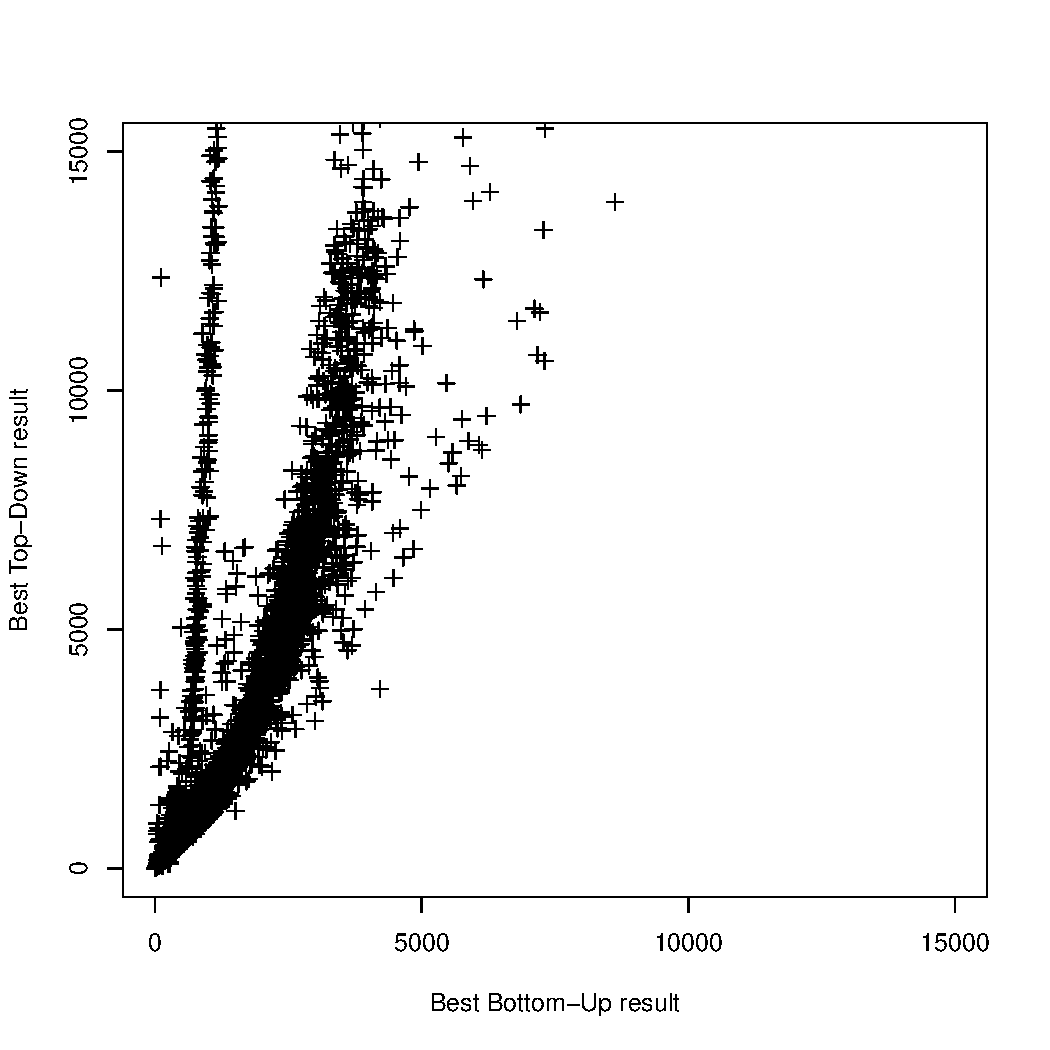
\includegraphics[scale=0.5]{figures/td_vs_bu.pdf}
	\caption{Space measures of best Bottom-Up and Top-Down result}
	\label{fig:BUvsTD}
\end{figure}

The Bottom-Up algorithm does not only produce better results, it is also much faster, as can be seen in the last column of Table \ref{tab:results}. 
Most likely, the reason is the number of comparisons made by the algorithms. 
For Bottom-Up the set $N$ of possible choices consists of the premises of a single node only, i.e. $|N| \in \{0,2\}$.
For Top-Down the set $N$ is the set of currently pebbleable nodes, which can be large (e.g. for a perfect binary tree with $2n -1$ nodes, initially $|N| = n$). 
Possibly for some heuristics, Top-Down algorithms could be made more efficient by using, instead of a set, an ordered sequence of pebbleable nodes together with their memorized heuristic evaluations.

Unsurprisingly the radius used for the Distance Heuristic has a severe impact on the speed, which decreases rapidly as the maximum radius increases. 
With radius 5, only a few small proofs were processed in a reasonable amount of time.

On average the smallest space measure of a proof is 44.1 times smaller than its length. 
This shows the impact that the usage of deletion information together with well constructed topological orders can have. 
When these techniques are used, on average 44.1 times less memory is required for storing nodes in memory during proof processing.


%\section{Future Work}
\label{sec:pebblingfuturework}

Most of the heuristics rely on basic information of the nodes.
More sophisticated combinations of characteristics of nodes and the proof as a whole as well as other sources of information could be used to come up with new and more successful heuristics.
For example information about the proof could already be used and stored during proof creation and conflict graph analysis.
Furthermore, different sequences of heuristics to decide ties could be evaluated.

The problem of constructing pebbling strategies with the pebbling number of the proof could be formulated as a constraint programming problem instance.
The encoding would be similar to the SAT encoding, but might not suffer from the high number of clauses.

Implementing the proposed methods directly into a SAT- or SMT solver would produce proofs with small space requirements right away without the need to post process it.
It would be interesting to see, whether our method can meet the high standards that solvers have to computation speed.

In the introduction the proof format DRAT was mentioned.
This proof format provides the possibility to output deletion information.
Comparing our deletion information with deletion information produced by some SAT or SMT solver, while keeping track of the maximum space required using this information, would show whether our method performs well w.r.t. methods used in solvers.

%%%%%%%%%%%%%%%%%%%%%%%%%%%%%%%%%%%%%%%%%
%%% Conclusion %%%%%%%%%%%%%%%%%%%%%%%%%%
%%%%%%%%%%%%%%%%%%%%%%%%%%%%%%%%%%%%%%%%%
%\chapter{Conclusion}
%\label{ch:conclusion}
%%%%%%%%%%%%%%%%%%%%%%%%%%%%%%%%%%%%%%%%%

\section{Conclusion}
\label{sec:conclusion}

The problem of compressing proofs in space has been reduced to finding strategies in a Pebbling Game, for which finding the optimal strategy is known to be NP-complete.
Therefore, two heuristic algorithms for compressing proofs in space have been conceived. The experimental evaluation clearly shows that the so-called Bottom-Up algorithms are faster and compress more than the more natural, straightforward and simple Top-Down algorithms. Both kinds of algorithms are parametrized by a heuristic function for selecting nodes. The best performances are achieved with the simplest heuristics (i.e. Last Child and Number of Children). More sophisticated heuristics provided little extra compression but cost a high price in execution time. Future work could investigate heuristics that take advantage of the particular shape of proofs generated by analysis of conflict graphs.
Furthermore, the methods could be implemented directly into a SAT- or SMT-solver to provide proofs with small space right away.

\vspace{-5pt}
\paragraph{Acknowledgments:} We would like to thank Armin Biere for clarifying why resolution chains are not left-associative in the TraceCheck proof format.

\vspace{-5pt}



%\newpage

\marginpar{ToDo: fix overfull hboxes}

\bibliographystyle{splncs}
\bibliography{jabref_references}


\end{document}